
\section{Zero-Coupon Yields}

\noindent The data I intend to use in this thesis is the zero-coupon bond yield data from Norges Bank, found on their website or at the link in Appendix \ref{ch:links}. The data includes the yields, or interest rates, of zero-coupon bonds with different maturities (tenors/lifetimes). The dataset has $2591$ distinct dates, and for each date it has the following tenors: $0.5$, $0.75$, $1$, $2$, $3$, $4$, $5$, $6$, $7$, $8$, $9$, and $10$. The tenors are denoted in years, so if an interest rate has a tenor of $0.5$, it means that the bond associated with that interest rate has a maturity of $6$ months. All the interest rates are annualized, meaning they are the interest rates for an entire year. The dates ranges from January $2$, $2015$, to April $30$, $2025$, and each year has approximately $252$ trading days. As a premise in this analysis I will assume that a year consist of $252$ days.



\begin{figure}[H]
    \centering
    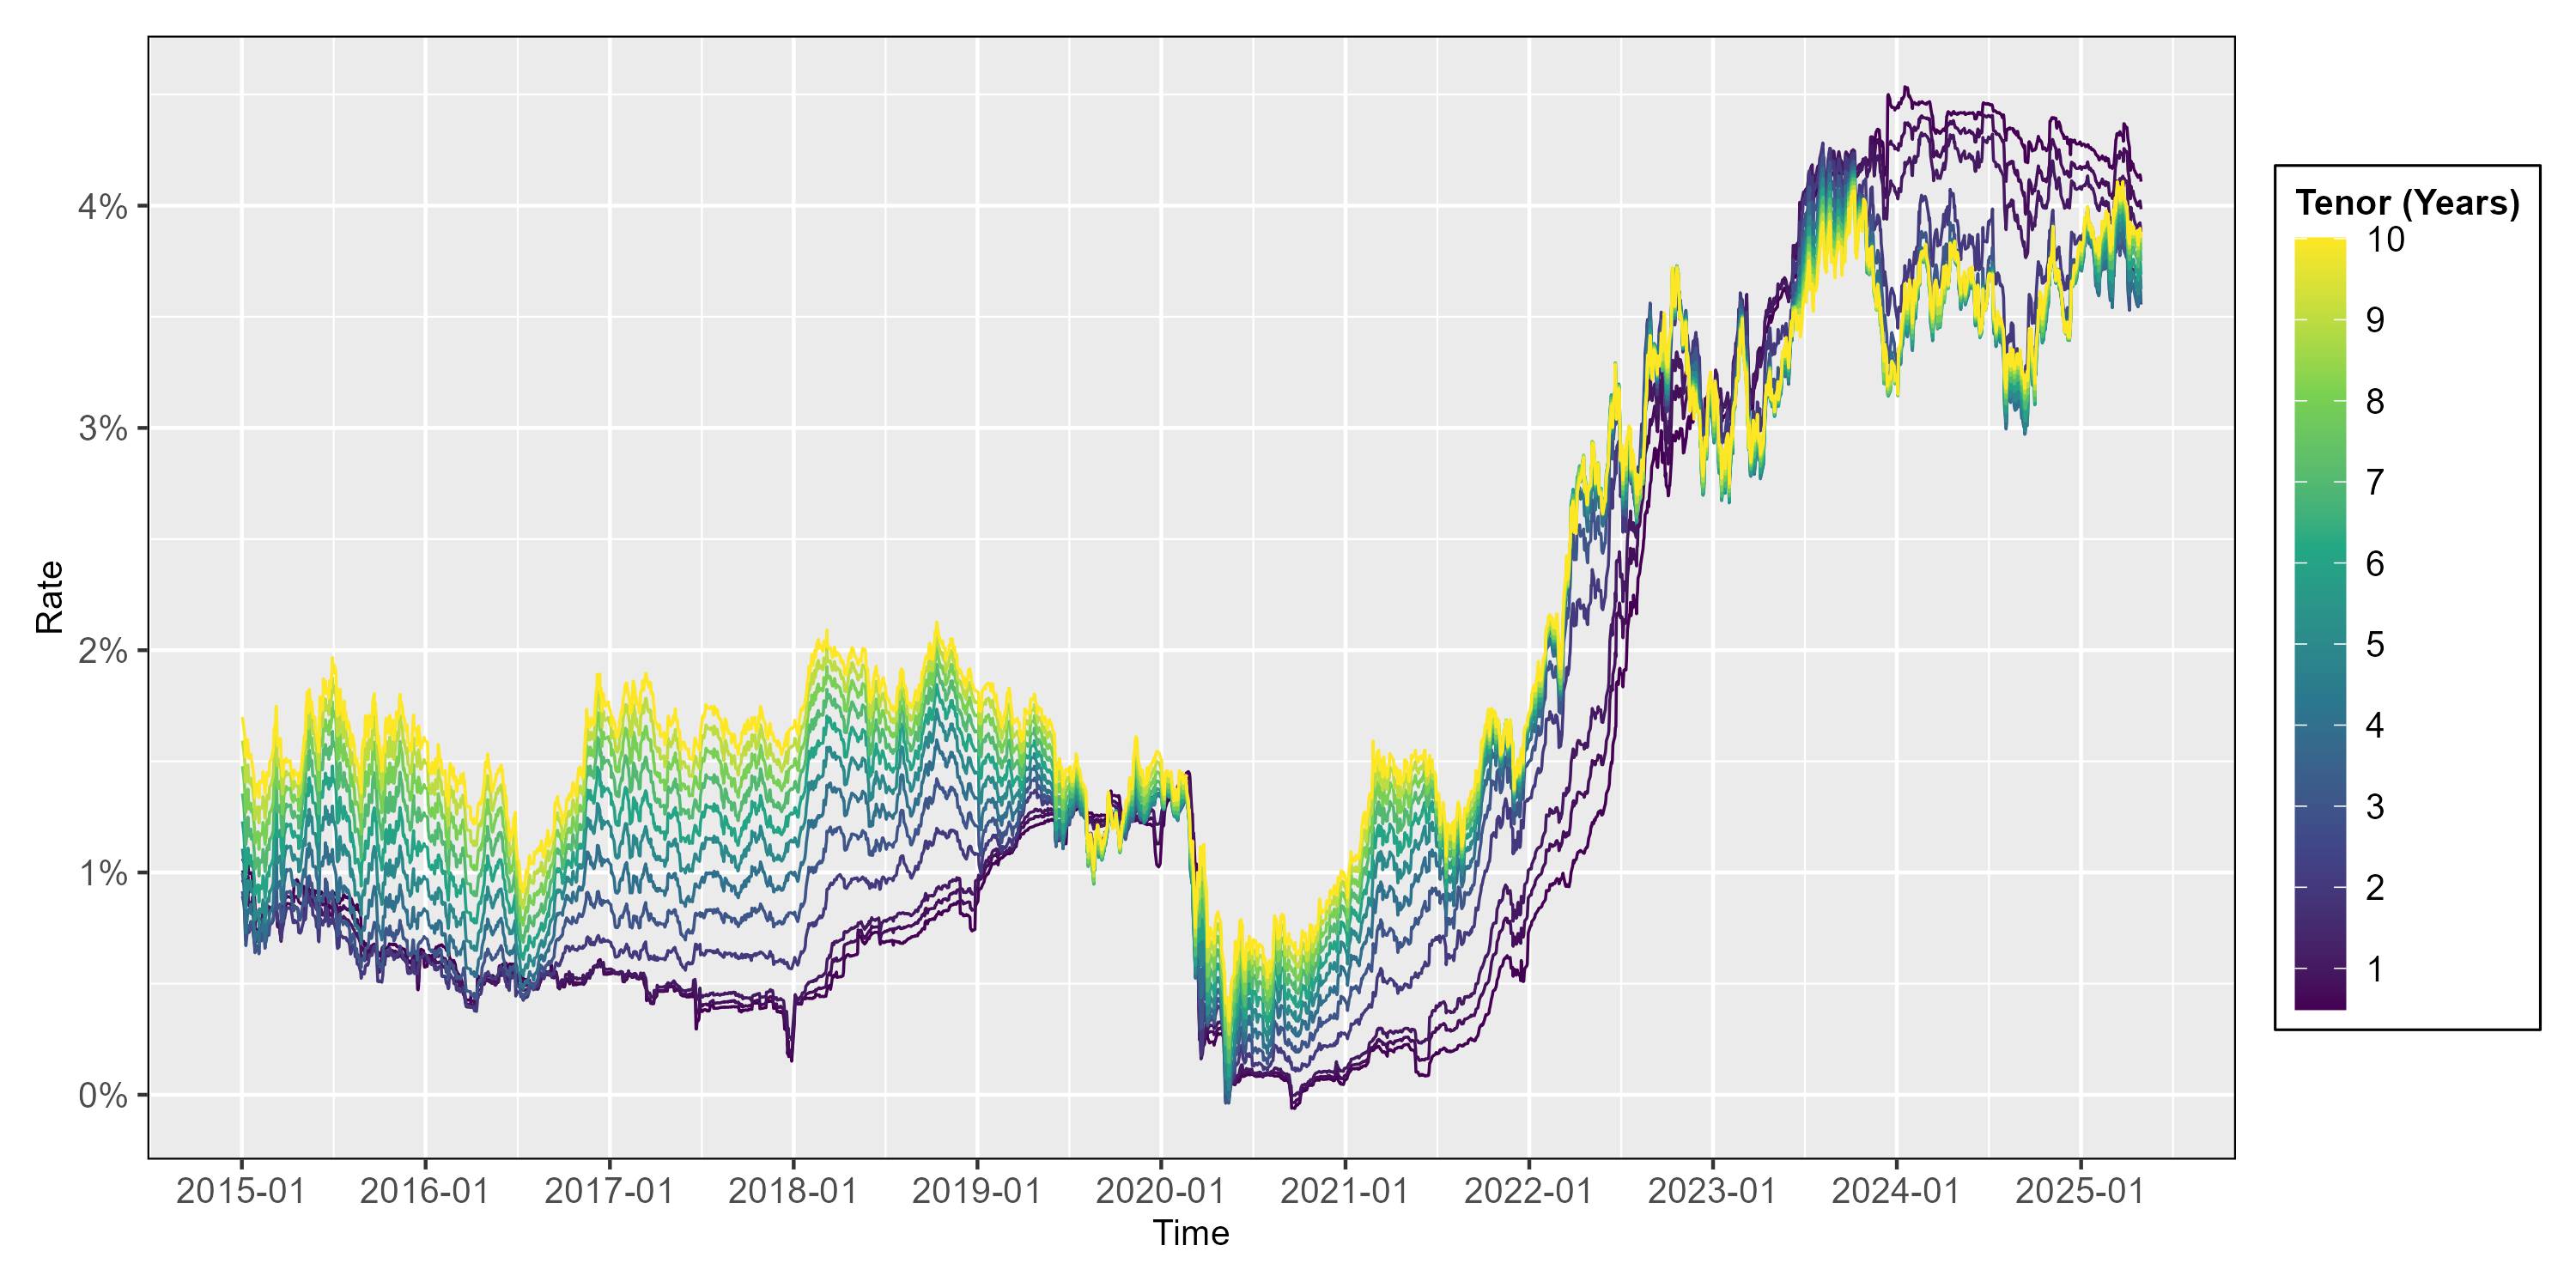
\includegraphics[width=.95\linewidth]{Figures/Interest Rates/zero_coupon_yields_dates_time_plot.png}
    \caption[Zero-Coupon Yields]{Zero-coupon yields, starting January $2$, $2015$, and ending April $30$, $2025$.}
    \label{fig:zero-coupon yields time}
\end{figure}

\vfill

\newpage

\section{Data Visualization}

\noindent The interest rates are plotted in Figure \ref{fig:zero-coupon yields time} on the previous page, and the differenced interest rates are plotted in Figure \ref{fig:differenced zero-coupon yields time} on the next page. Figure \ref{fig:zero-coupon yields time} helps with visualizing the interest rates over time and Figure \ref{fig:differenced zero-coupon yields time} helps with visualizing the volatility of the interest rates over time. The data can be decomposed into three periods.

\begin{enumerate}
    \item Period $1$ starts January $2$, $2015$, and ends February $28$, $2020$. This period is characterized with low and somewhat stable interest rates. There are a few spikes in the volatility but not as much as later dates. This period ends because of the COVID-19 pandemic, which ravaged the world at the beginning of $2020$, causing job losses and financial turmoil \cite{norges_bank_covid}.
    \item Period $2$ starts March $2$, $2020$, and ends June $30$, $2023$. This period is characterized with a rapid fall in interest rates followed by a slowly rising interest rates with low volatility. At the end of this period we see higher volatility. The rapid fall was caused by Norges Bank, which lowered the policy rate to help stimulate the economy. With the increasing job losses people tried to save as much money as possible, so to make people spend money Norges Bank tried to make it cheaper to borrow money \cite{nrk_covid}. The interest rates slowly began to rise because of the inflation caused by the increasing spending. This led the interest rates to a $10$-year high.
    \item Period $3$ starts July $3$, $2023$, and ends April $30$, $2025$. For interest rates with short tenors, this period is characterized with high and stable interest rates. For interest rates with longer tenors, it is characterized with lower interest rates with higher volatility. I have plotted the interest rates from this period in Figure \ref{fig:zero-coupon yields third phase dates time}, which shows the characteristics better. The interest rates with short and long tenors are closer together at the end of period $3$ than they were the previous year. The yield curve and the extrapolated yield curve as of April $30$, $2025$, can be seen plotted in Figure \ref{fig:current zero-coupon yield curve}. We can see that interest rates in the middle are lower than interest rates with short and long tenors. This figure also shows that the NS model is not perfect, but the estimated interest rates are close to the real values. The longest tenors shows a slight deviation, but this is small.
\end{enumerate}

I will only use the data from period $3$ because the other periods include movements we are not currently experiencing as of April $30$, 2025. If I included data from periods $1$ and $2$ it would give lower volatilities, because those periods has a lower volatility than period 3. From looking at Figure \ref{fig:zero-coupon yields third phase dates time} I expect that the volatilities fitted will be much lower for short tenors because they are much more stable.

\newpage

\vfill

\begin{figure}[H]
    \centering
    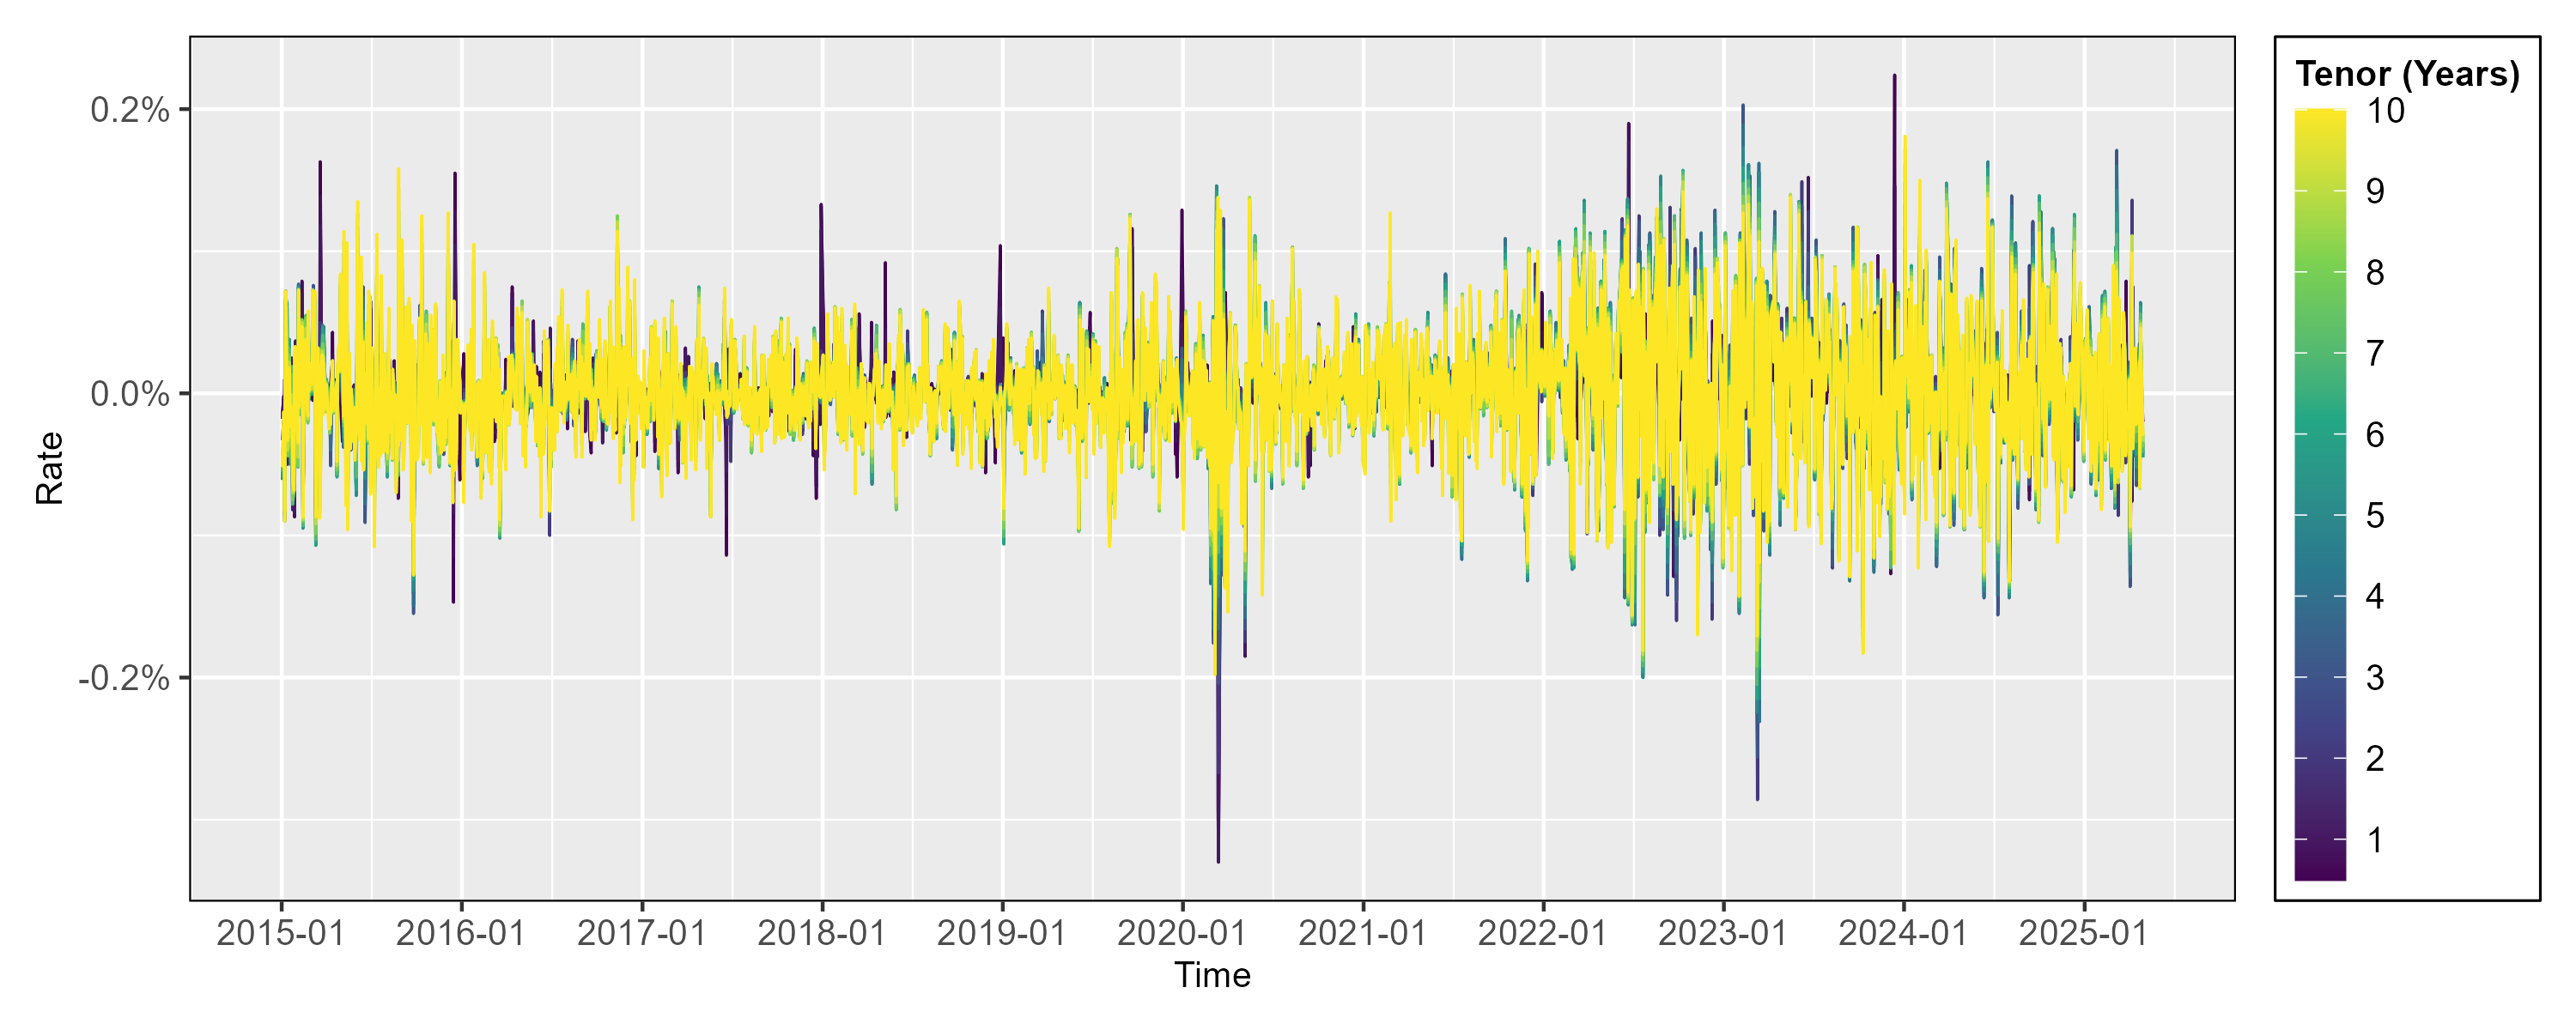
\includegraphics[width=.95\linewidth]{Figures/Interest Rates/zero_coupon_yields_dates_small_diff_time_plot.png}
    \caption[Differenced Zero-Coupon Yields.]{Differenced zero-coupon yields, starting January $2$, $2015$, and ending April $30$, $2025$.}
    \label{fig:differenced zero-coupon yields time}
\end{figure}

\vfill

\begin{figure}[H]
    \centering
    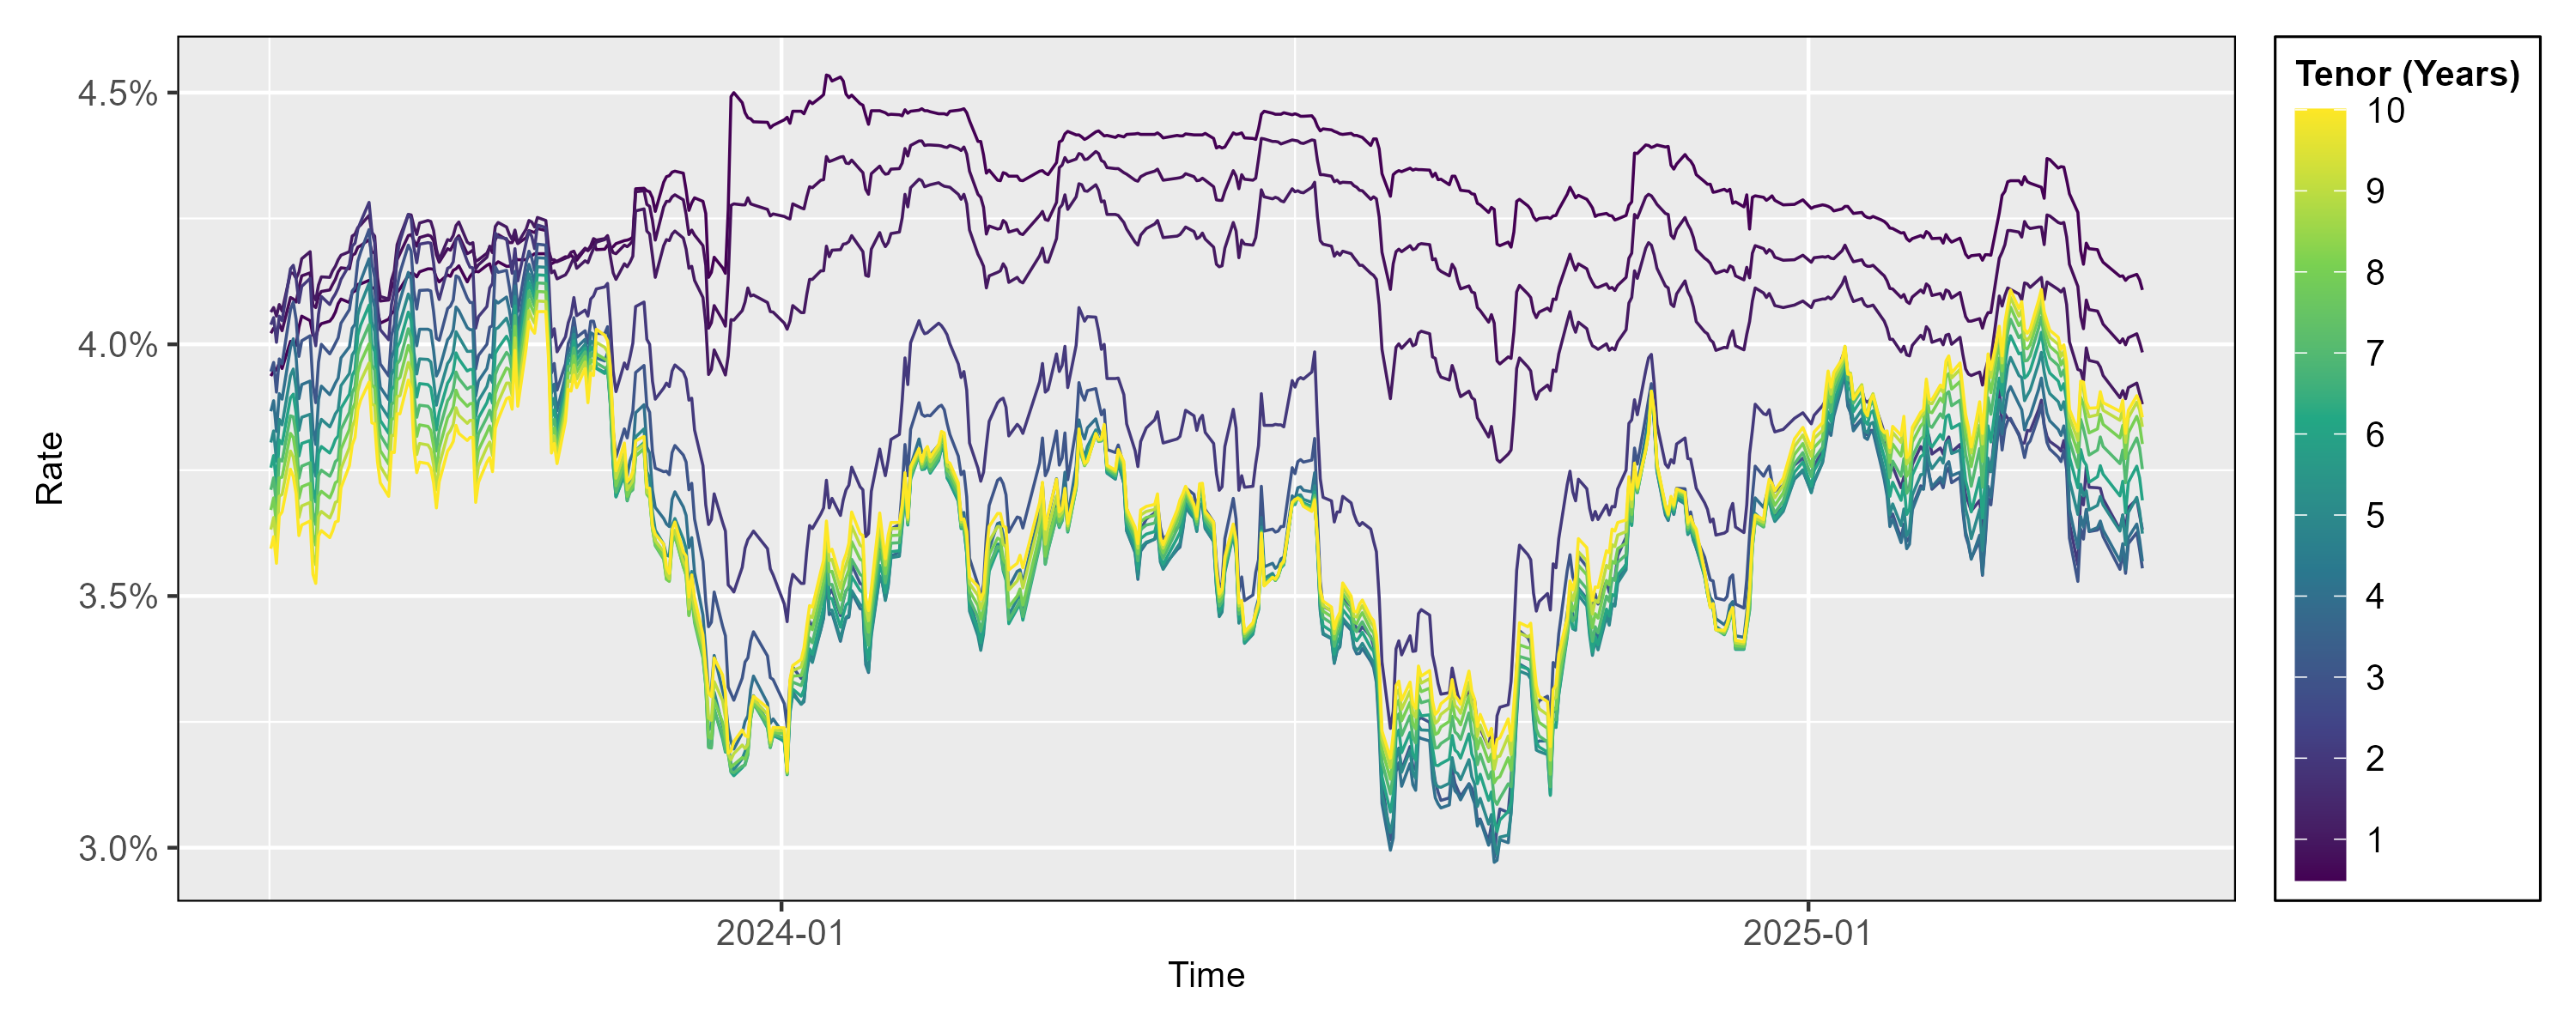
\includegraphics[width=.95\linewidth]{Figures/Interest Rates/zero_coupon_yields_phase_3_dates_small_time_plot.png}
    \caption[Zero-Coupon Yields, Period 3]{Zero-coupon yields, Period 3, starting July $3$, $2023$, and ending April $30$, $2025$.}
    \label{fig:zero-coupon yields third phase dates time}
\end{figure}

\vfill

\begin{figure}[H]
    \centering
    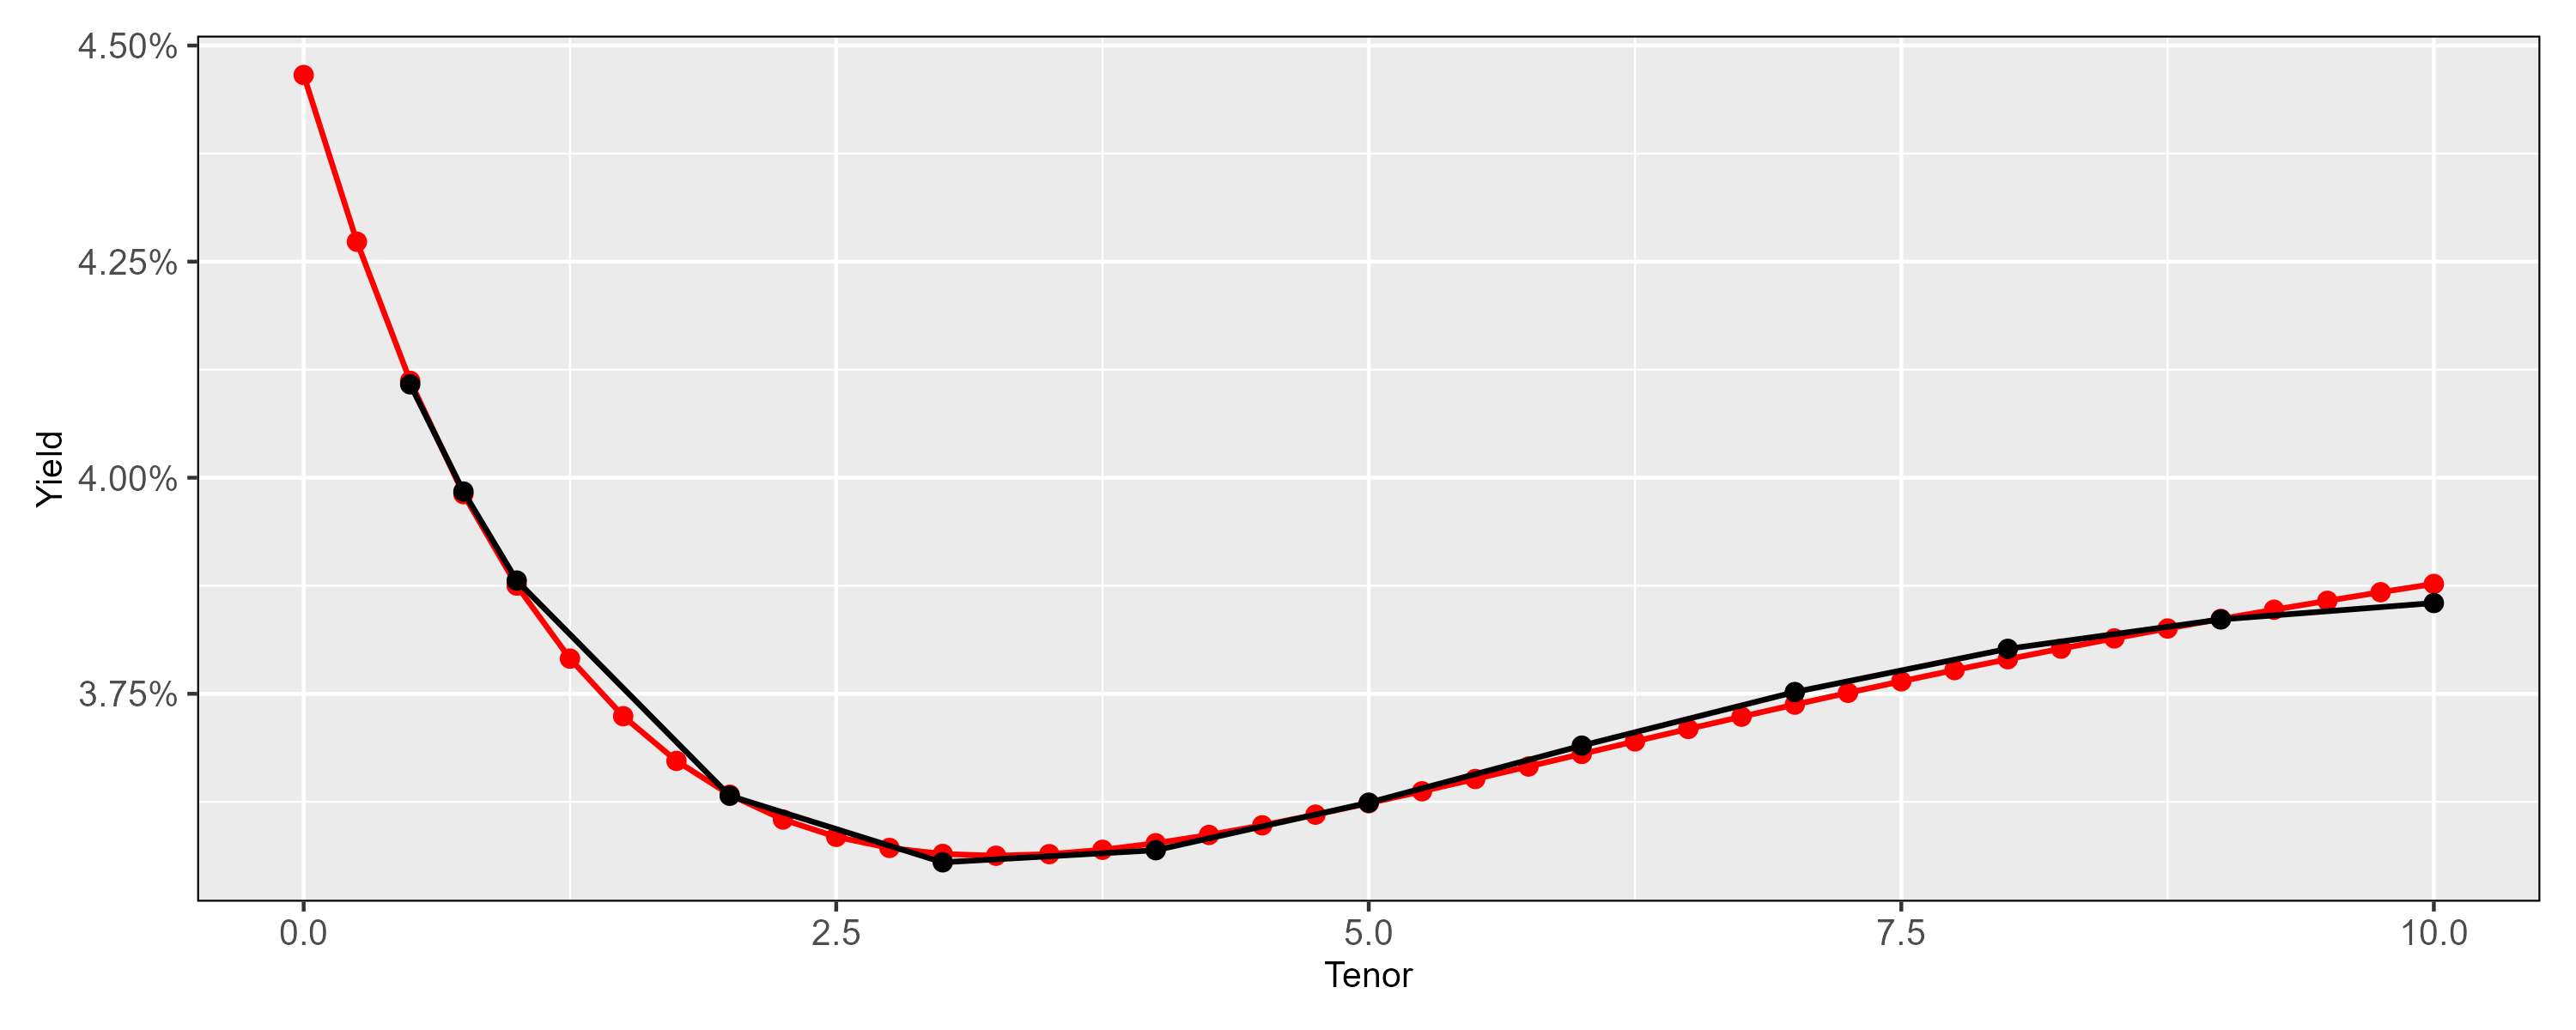
\includegraphics[width=.95\linewidth]{Figures/Interest Rates/current_zero_coupon_yields_w_extrapolated_curve_yield_curve.png}
    \caption[Current Zero-Coupon Yield Curve.]{Zero-coupon yield curve as of April 30 2025. The solid \textbf{black} $\bigl($\textbf{---}$\bigr)$ line is the yield curve for the data. The solid \textbf{red} $\bigl($\textcolor{red_}{\textbf{---}}$\bigr)$ line is the extrapolated yield curve using the NS model.}
    \label{fig:current zero-coupon yield curve}
\end{figure}

\vfill

\newpage

The correlation matrix of the data in Figure \ref{fig:zero-coupon yields third phase dates time} is shown in Figure \ref{fig:corr plot}. From this we can see that the $0.5$-, $0.75$-, $1$-year interest rates are highly correlated with each other. We also see that the rest of the interest rates are highly correlated with each other. This indicates that we have two different movements in the data, one movement for the short tenors, and one movement for the longer tenors.

\begin{figure}[H]
    \centering
    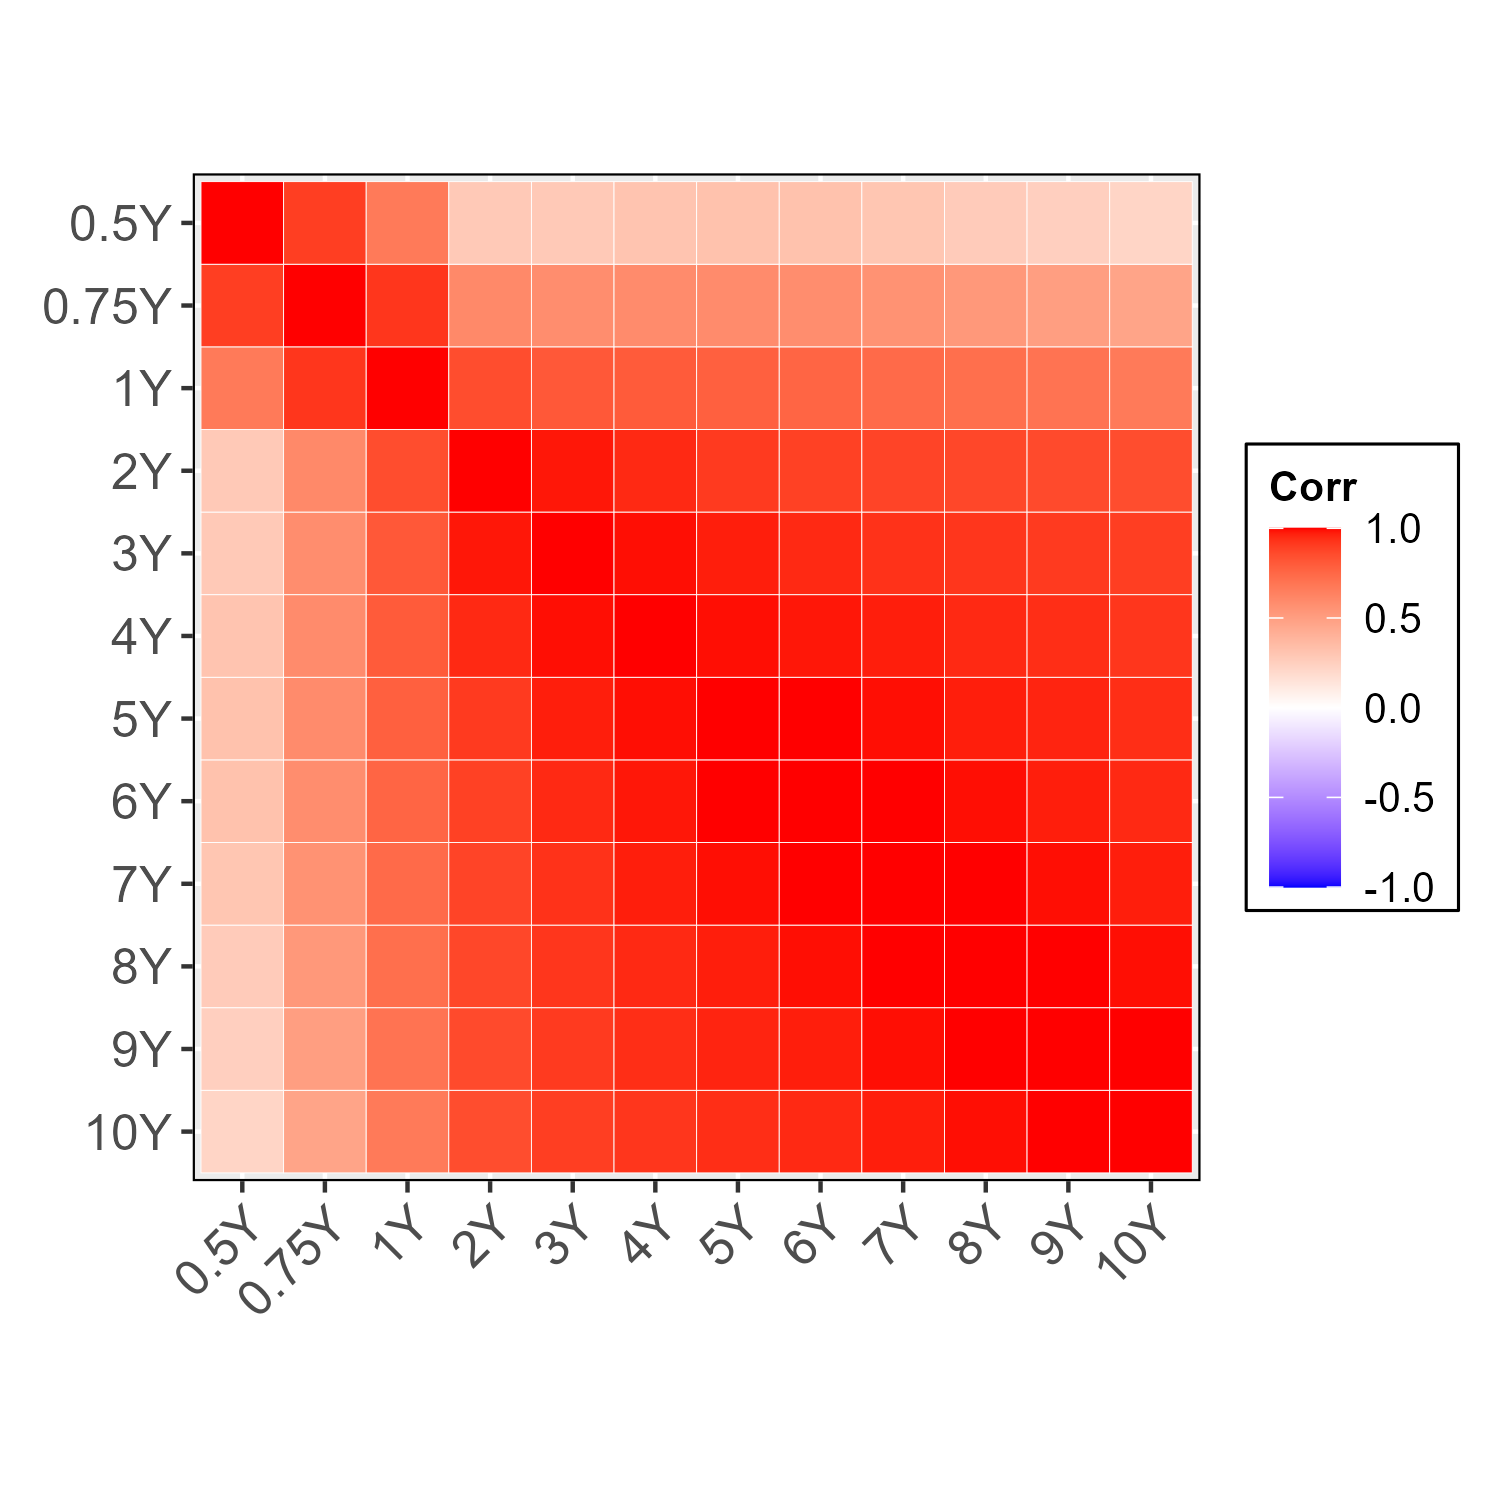
\includegraphics[width=0.5\linewidth]{Figures/Correlation/zero_coupon_yields_phase_3_correlation.png}
    \caption[Correlation plot, Period $3$.]{Correlation plot, period $3$.}
    \label{fig:corr plot}
\end{figure}
